
\documentclass[paper=a4, fontsize=12pt]{scrartcl} 

\usepackage[left=2.7cm,right=2.7cm,top=2.5cm,bottom=2.5cm]{geometry}
\usepackage[utf8]{inputenc} 
\usepackage{mathpazo} % Palatino font
\usepackage{microtype}
\usepackage[T1]{fontenc}
\usepackage{fourier}
\usepackage[english]{babel}
\usepackage{amsmath,amsfonts,amsthm}
\usepackage{lipsum}
\usepackage{caption}
\usepackage{subcaption}
\usepackage{graphicx}
\usepackage{float}
\usepackage{blindtext} 
\usepackage[hidelinks]{hyperref}
\usepackage{sectsty}
\usepackage{natbib}
\usepackage{caption} 
\usepackage{ragged2e}

\sectionfont{\centering \normalfont\scshape}
\subsectionfont{\centering \normalfont \scshape}
\subsubsectionfont{\normalfont\itshape}

% note divider
\newcommand{\notedivider}{%
	\vspace{4pt}%
	{\hrule height 0.4pt}%
	\vspace{6pt}%
	{\hrule height 0.4pt}
	\vspace{6pt}
}

\captionsetup{font={normal}, 
	labelfont=bf} % sans serif figure and table captions

\usepackage{fancyhdr} % Custom headers and footers
\pagestyle{fancyplain} % Makes all pages in the document conform to the custom headers and footers
\fancyhead[L]{} % No page header - if you want one, create it in the same way as the footers below
\fancyhead[R]{}
\fancyhead[C]{}
\fancyfoot[L]{} % Empty left footer
\fancyfoot[C]{\thepage} % Empty center footer
\fancyfoot[R]{} % Page numbering for right footer
\renewcommand{\headrulewidth}{0pt} % Remove header underlines
\renewcommand{\footrulewidth}{0pt} % Remove footer underlines
\setlength{\headheight}{13.6pt} % Customize the height of the header

%\numberwithin{equation}{section}
%\numberwithin{figure}{section} 
%\numberwithin{table}{section} 
\setlength\parskip{4pt}
\setcounter{secnumdepth}{3}
\setcounter{tocdepth}{3}


\begin{document}
	
	\setcitestyle{authoryear,square,aysep={,},yysep={;}} %bloody hell this took a while but use this for commas between author, year with natbib
	\bibliographystyle{apalike}
	%\renewcommand{\bibfont}{\sffamily\footnotesize}
	
	%----------------------------------------------------------------------------------------
	%	TITLE PAGE
	%----------------------------------------------------------------------------------------
	
	\begin{titlepage} % Suppresses displaying the page number on the title page and the subsequent page counts as page 1
		\vspace*{5em} % star for top of page
		\newcommand{\HRule}{\rule{\linewidth}{0.5mm}} % Defines a new command for horizontal lines, change thickness here
		
		\centering % Centre everything on the page
		
		
		\textsc{\LARGE University of Bristol}\\[1.5cm] % Main heading such as the name of your university/college
		\vspace{-3em}
		\textsc{\Large MSc Bioinformatics}\\[0.5cm] % Major heading such as course name
		\vspace{3em}
		
		%\HRule\\[0.4cm]
		
		{\Large\bfseries Evaluating Evapotranspiration Generalisation Under a Changing Climate using Machine Learning NOTES}\\[0.4cm] % Title of your document
		
		\vspace{3em}
		
		%	\HRule\\[1.5cm]
		
		%------------------------------------------------
		%	Author(s)
		%------------------------------------------------
		
		\begin{minipage}{0.4\textwidth}
			\begin{flushleft}
				\large
				\textit{Author}\\
				Archie \textsc{Benn} % Your name
			\end{flushleft}
		\end{minipage}
		~
		\begin{minipage}{0.4\textwidth}
			\begin{flushright}
				\large
				\textit{Supervisor}\\
				Professor Martin \textsc{De Kauwe} % Supervisor's name
			\end{flushright}
		\end{minipage}
		
		\vspace{5em}
		\begin{abstract} 
			{\noindent{\textsc{Abstract} (The abstract has a  maximum of 200 words})}
			\newline
			%\lipsum[1-10][1-20]
			
			\begin{itemize}
				\item Summary of background on ET/ML methods and FLUXNET 
				\item Overall aim of the project 
				\item Proposed approach for the project
			\end{itemize}
			
			\vspace{1em}
			\textit{\textbf{Key words:}} Machine Learning, FLUXNET, Evapotranspiration.\\
			\textit{\textbf{Word count:}} 3000
		\end{abstract}
	\end{titlepage}
	
	\newpage
	\tableofcontents
	\newpage
	
	%------------------------------------------------
	% LIT REVIEW
	%------------------------------------------------
	
	\section{Literature Review ($\sim$ 1750 words)}
	\subsection{Evapotranspiration and The Water Cycle \\ \textit{(Why does the water cycle matter?)}}
	\subsubsection{Evapotranspiration} 
	\begin{itemize}
		\item Overview of evapotranspiration (ET) (from \citep{wang2012review}):
		\begin{equation}
			ET = Transpiration + E_{Vegetation} + E_{Soil}
		\end{equation}
		\item How this plays into the water cycle globally/regionally/in watersheds more generally.
		\item Drivers of ET e.g Leaf Area index (LAi), Vapour pressure deficit (VPD), precipitation, air temperature etc.
		\item Importance and applications of ET predictability
	\end{itemize}
	\notedivider
	\textbf{From \citep{amani2023review}:}
	
	
	
	\newpage
	\notedivider
	\subsubsection{Eddy Covariance}
	\begin{itemize}
		\item Overview of eddy covariance and briefly how flux tower data collection
		\item How this relates to ET
		\item FLUXNET and how sites are grouped (region and vegetation types)
	\end{itemize}
	\notedivider
	
	\newpage
	\subsection{The Changing Climate\\ \textit{(How is the water cycle changing?)}} 
	\notedivider
	\subsubsection{Climate Change}
	\begin{itemize}
		\item Overview of climate change and effects on water cycle via carbon dioxide levels/temp. etc.
		\item How these could link to factors such as changing ET
		\item Issues of rapidly changing ET/inability to predict accurately
	\end{itemize}
	\notedivider
	
	\newpage
	\subsection{Evapotranspiration Prediction\\ \textit{(What don't we know and what are the issues?)}}
	\notedivider
	\subsubsection{Contemporary ET Prediction Methods}
	\begin{itemize}
		\item Very brief description of non-ML methods for background e.g from \cite{xu2018evaluating}
		\item Disagreement of current satellite and process-based models (between and within)- lack of theory
		\item Lead into ML methods
	\end{itemize}
	\notedivider
	
	\newpage
	\notedivider
	\subsubsection{Machine Learning Models for ET Prediction}
	\begin{itemize}
		\item Brief overview of current ML methods in ET prediction
		\item Performances of different models in the literature 
	\end{itemize}
	\notedivider

	\newpage
	\subsection{Project Scope and Machine Learning Applicability\\ \textit{(What is the case for using ML here?)}}
	\notedivider
	\subsubsection{Project Scope}
	\begin{itemize}
		\item Address explicit question being asked in project 
		\item "Do predictive ET ML models trained on historic FLUXNET data have a loss of performance under new climate conditions?"
	\end{itemize}
	\notedivider
	
	\newpage
	\notedivider
	\subsubsection{Why is ML applicable here?}
	\begin{itemize}
		\item Why is ML important for this specific question?
		\item Include why this is addressable now
	\end{itemize}
	\notedivider
	
	%------------------------------------------------
	% PROJECT PLAN
	%------------------------------------------------
	
	
	\newpage
	\section{Research Project Plan ($\sim$ 1000 words)}
	\subsection{Overall Project Aim}
	\notedivider
	\subsubsection{Aims}
	\begin{itemize}
		\item Overview of how this project will answer the question/area proposed at end of introduction.
	\end{itemize}
	\notedivider
	
	\newpage
	\subsection{Methods Overview}
	\notedivider
	\subsubsection{Data Acquisition and Selection}
	\begin{itemize}
		\item How the data will be accessed and stored (FLUXNET).
		\item Time period (requires long term sites) and geographical location of data selected for modelling.
		\item Why these were selected and appropriate? (in terms of location/times, not specific structure).
	\end{itemize}
	\notedivider
	
	\newpage
	\notedivider
	\subsubsection{Feature Engineering}
	\begin{itemize}
		\item Selection of data features for use in training and why.
		\item How these were removed or adapted
		\item Why are these features appropriate?
	\end{itemize}
	\notedivider
	
	\newpage
	\subsubsection{ML Model Setup and Training}
	\begin{itemize}
		\item How the data will be accessed and stored (remote sensing and FLUXNET).
		\item Explanation of model(s) selection (type of ML method)
		\item e.g If including LAi vs. not with other parameters kept identical across 2 models.
		\item Overview of model parameters (- might be too much detail?) and how each are trained.
		\item Why are these model choices/parameters appropriate for this task?
		\item Target features: FLUXNET latent heat flux (ET approximation)
		\item Predictor features: Meteorological data (from FLUXNET and others like LAi)
	\end{itemize}
	\notedivider
	
	\textbf{From \citep{xu2018evaluating}:} \textit{``ET was trained and predicted under different land cover types with the following equation:''}
	\begin{equation}
		ET_i = M\left(R_{si},\sum_{i=30}^{i}P_{i},LAI_{i},T_{ai},RH_{i}\right)
	\end{equation}
	
	\textit{``...where $M$ is the training model; $ET_i$ is the target variable; Solar radiation ($R_s$), Precipitation( $P$), Leaf area index ($LAI$), Air temperature ($T_a$), and relative humidity ($RH$) are the explanatory variables; and $P$ is the cumulative precipitation for the 30-day period prior to $i$th day. The subscript $i$ stands for $i$th day.''}
	
	\newpage
	\subsubsection{ML Model Evaluation}
	\begin{itemize}
		\item Testing methods on unseen/held out historical (same as training e.g 5-20 years old) validation sets
		\item Comparison to other predictive models e.g in FLUXCOM
		\item Overall evaluation of model predictability on historical data
	\end{itemize}
	\notedivider
	
	\textbf{From \citep{xu2018evaluating}:} \textit{``The global k-fold testing was adopted to examine the performance of each machine learning method. In this study, 36 sites (65 site years) of flux tower observations were divided into k parts (k = 10 herein). In each training, k 1 parts of data were used as the training data, and the kth part of data was used as the validation data. The cross-validation process was repeated k times (all the data set should be trained and validated), and the results of the evaluation index were then averaged as the assessing results. Although k-fold testing is time consuming for operational application, the data are fully used and the model can lead to more accurate results than the residual testing method.''}
	
	\begin{figure}[H]
		\centering
		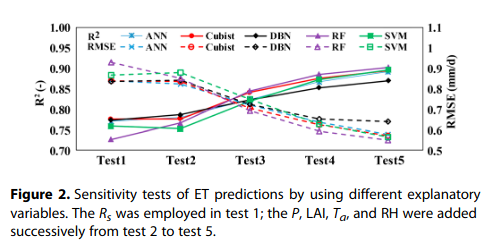
\includegraphics[width=0.75\textwidth]{photos/xu2018.png}
		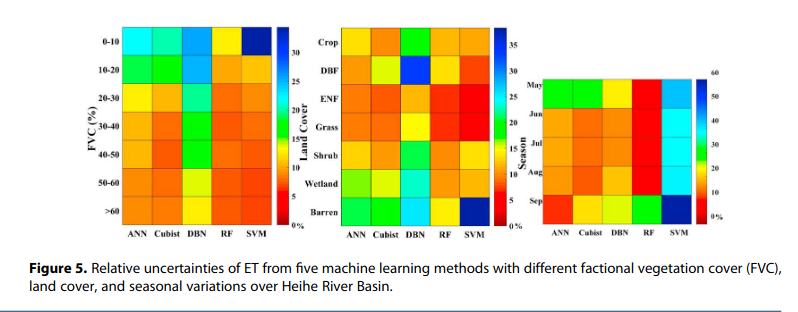
\includegraphics[width=0.75\textwidth]{photos/xu2018_2.png}
		\captionsetup{justification=centering}
		\caption{Examples of some comparisons and testing of model performance in \cite{xu2018evaluating}}
		\label{fig:plddt}
	\end{figure}
	
	
	\newpage
	\notedivider
	\subsubsection{ML Model Predictions}
	\begin{itemize}
		\item Predictions made on unseen and more recent data (e.g last 5 years)
		\item Overall evaluation of model predictability on recent data
	\end{itemize}
	\notedivider
	
	\newpage
	\subsection{Gantt Chart}
	
	\begin{figure}[H]
		\centering
		
\includegraphics[width=\textwidth]{gantt/gantt1.png}
		\captionsetup{justification=Centering}
		\caption{A proposed Gantt Chart for the duration of this project.}
		\label{fig:gantt}
	\end{figure}
	
	
	
	
	%------------------------------------------------
	% RISK REGISTER
	%------------------------------------------------
	
	\newpage
	\section{Risk Register ($\sim$ 250 words)}
	\begin{itemize}
		\item 4-5 risks at about 50 words each
		\item Data access issues, overfitting, data gaps etc.
	\end{itemize}
	
	\newpage
	\section{Papers}
	\subsection{Evaluating Different Machine Learning Methods for Upscaling Evapotranspiration from Flux Towers to the Regional Scale \citep{xu2018evaluating}
	}
	\subsubsection{Introduction}
	\begin{itemize}
		\item upscale ET from 36 flux tower sites (65 site years) to regional scale
		\item ML methods: artificial neural network, cubist, deep belief network, RF, and support vector networks
		\item essentially took these methods and trained on those 65 years...
		\item then applied to estimate on each grid cell within a watershed between 2012-2016  
		\item deep belief was worst, others had similar performance, and RF had lowest relative uncertainty
		\item ML performed better on densely vegetated conditions than barren/sparse land
		\item "Satellite sensors detecting two-dimensional information of land surface become an effectiv>
		\item 1) predictive equations which link ET observations (flux towers) to vegetation indices 
		\item 2) "geostatistical methods" based on kriging theoretical framework  
		\item 3) using semi-theoretical or running theoretical methods  
		\item 4) using ML methods  
		\item "All of these studies (lists ML methods for ET flux predictions) trained the machine learni>
	\end{itemize}
	
	\subsubsection{Methods}
	\begin{itemize}
		\item went over the 5 ML methods  
		\item study area and data sets
		\item looks at specific river basin in China  
		\item goes over how upstream/midstream/downstream areas in basin are characterised by weather and vegetation like '...mountaineous areas with relatively high precip and mainly covered by grassl>
		\item hydrometeorology observation network was set up within the basin in 2008-2011  
		\item ET observations from eddy covariance (EC) towers (flux towers) was used to test the ML models performance   
	\end{itemize}
	
	\subsubsection{Results}
	\begin{itemize}
		\item Models were sensitive to all the variables in the models, so including all was beneficial.
		\item performance of the 5 models was tested against observed EC data 2012-2016 using R-squared plot  
		\item all 5 rough;y followed 1:1 line, with R-2 values of 0.87-0.89  
		\item RMSE was also calculated alongside MAPE (?)  
		\item so performance evaluated using R-2, RMSE, and MAPE  
		\item as all relatively similar, relative uncertainty was important with 3 cornered hat method  
		\item RF model slightly outperformed the other ML methods based on R2, MAPE, RMSE and relative uncertainties   
		\item therefore RF model was taken forward to predict 2012-2016 over river basin  
	\end{itemize}
	
	\subsubsection*{Limitations and Unresolved}
	\begin{itemize}
		\item Heihe River Basin, the 36 site observations (65 site years; sample number is 65 site year × 365 day/year = 23,725) is not large enough for deep belief network (DBN) model training. Thus, the DBN algorithm underperformed other four algorithms in this study.
		\item larger dataset than the one used here would be better for deep learning models  
		\item ET is also a function of other variables, such as land surface temperature, wind speed, and soil type (or water storage capacity) which were not included here 
		\item However, wind speed increased RMSE here, soil type couldn't be included due to a large desert area in the basin, and cloud contamination meant  LST was not included either
		\item Models didn't match observations perfectly, largely due to: \newline 
		1) ML models simply learn statistical patterns, rather than causal relationships between the included variables ie. can predict well on average but can misrepresent underlying physics. \newline 
		2) truth/observation data isn't exact - EC measurements used here have an uncertainty of about 16\% (wang, 2015). Some mismatch between predictions and observed is expected even in a perfect model as comparing against an imperfect reference. \newline
		3) Higher unertainty in downstream region where there is greater complexity to the land cover types and varying irrigation etc. ML models struggle to capture that spatial complexity which leads to more uncertainty vs. more uniform landscapes.
		\item These 3 compound each other - an imperfect model which doesn't truly understand the physics trained on imperfect data and predicting on a heterogeneous (non-uniform) landscape will inevitable show mismatches.
		\item Models performed much better in vegetation than in barren land, and this is possibly due to the reduced LAi values degrading the models' performances and increasing uncertainties.
	\end{itemize}
	
	
	\subsubsection*{Conclusion/Suggestions}
	\begin{itemize}
		\item ML methods predict better over dense vegetation than sparse region here.
		\item Inclusion of land surface temperature and soil moisture content at fine resolutions could improve the ML performance for ET predictions.  
	\end{itemize}
	
	\subsection{A review of machine learning models and influential factors for estimating evapotranspiration using remote sensing and ground-based data \citep{amani2023review}}
	
	\subsubsection{Introduction}
	\begin{itemize}
		\item Accurate ET estimation is important in understanding ecological and hydrological processes, mitigating droughts, effective water use management/irrigation, and understanding relationship between atmosphere, hydrosphere, and biosphere.
		\item ET is a complex phenomenon influenced by a set of biophysical and environmental factors. Its estimation becomes more complicated in heterogeneous environments, demanding detailed data and accurate model calibration.
		\item ET (top equation) is controlled by factors such as vegetation type, fractional vegetation cover (FVC), phonological cycle, soil type, soil moisture, irrigation and drainage, meteorological conditions, and water management in croplands (i.e. maintaining soil moisture and irrigation management)
		\item ET estimation can be direct or indirect. Eddy covariance is direct (via Latent heat flux), and lysimeter is the most accurate but has issues such as expensive, hard to use, and associated with environmental degredation.
		\item Remote sensing data cannot provide a direct estimation of surface ET; instead, they estimate the retrievable surface parameters associated with ET, such as surface temperature, vegetation indices, and soil moisture.
		\item Point methods can provide ET measurements (e.g flux towers) on a local scale, but the direct measurement of ET on a global scale is impossible, as dense global coverage by such instruments is neither available nor feasible.
	\end{itemize}
	
	\subsubsection{Review Main Points}
	\begin{itemize}
		\item Accurate identification and selection of input data is key to developing an ML model; hence, one should always consider the input data in terms of availability and relevance. Variables affecting ET include climatic factors (maximum and minimum temperature, wind speed, relative humidity, duration, and intensity of solar radiation), soil properties (soil moisture, crop type, agricultural practices, soil texture), and plant properties (plant type, growth stage, leaf shape, total water potential within the leaf) (Allen et al., 1998).
		\item These two datasets act as complementary sources to increase the accuracy of ET estimation.
		\item Liu et al. (2022) investigated the effects of climate change, water fluctuations, and vegetation conditions on ET variation worldwide and identified temperature as the essential determinant of ET in most regions.
		\item The main advantage of ground observation data like FLUXNET is that it is ready to use without any preprocessing steps (Chia et al., 2020).
	\end{itemize}
	
		\begin{figure}[H]
		\centering
		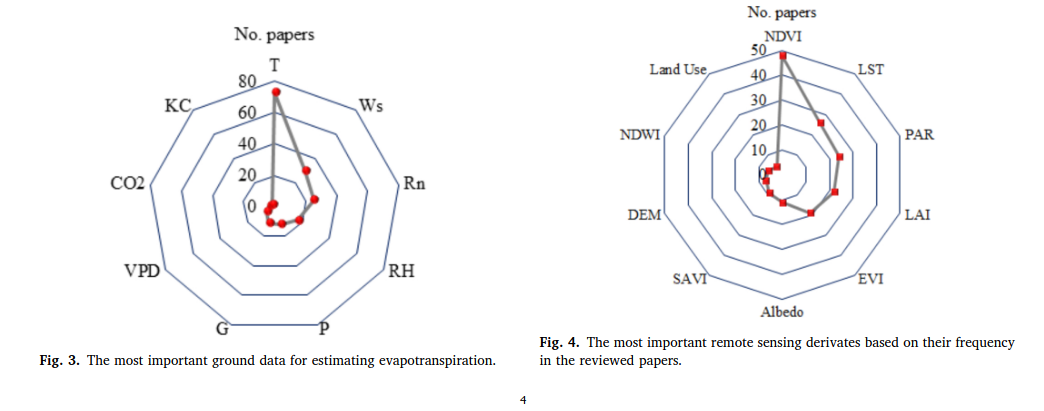
\includegraphics[width=0.95\textwidth]{photos/ground_rs.png}
		\captionsetup{justification=centering}
		\caption{Main variables for ground vs RS ET prediction in this review.}
		\label{fig:plddt}
	\end{figure}
	
	
	\subsubsection{Limitations and Unresolved}
	\begin{itemize}
		\item However, the use of tower/ground based data also has disadvantages; for example, meteorological station measurements only show the conditions of the tower and its proximity (Baldocchi, 2008; Yang et al., 2006), and setting up these is costly, leading to heterogenous distribution of these towers.
		\item In addition, the flux towers are not spatially well distributed, and this heterogeneous distribution leads to significant uncertainties in ET estimation at both regional and global scales (Li et al., 2018).
		\item ML models may struggle with extrapolation, meaning that they may not be able to generalize well beyond the data they were trained on.
		\item ML models may perform comparably or even better than complex physical methods, particularly for the large scale studies, but they do not have the interpretability that physical models do.
		\item accuracy of ML models depends on the quality of satellite and terrestrial data and the representativeness of the samples. There are sevHowever, the use of sucheral uncertainties associated with RS data. Some of these uncertainties include sensor noise, cloud cover, atmospheric interferences, shadows, limitations in spatiotemporal resolution, and satellite viewing angle. 
		\item Satellites with a higher temporal resolution usually have a lower spatial resolution, combining different sensors is necessary to obtain higher frequencies and better spatial resolution.
		\item Geographically, most studies have been conducted in China, the United States, and European countries because of the presence of FLUXNET towers and reliable data for model validation in those areas. Nonetheless, ET estimation in arid and semi-arid regions such as Africa, South Asia, the Middle East, Australia, and the Arctic, is very important, and climate problems and water crises are evident in these areas
	\end{itemize}
	
	
	\subsubsection{Conclusion/Suggestions}
	\begin{itemize}
		\item  1) Advances in RS technology have facilitated the continuous monitoring of biophysical variables affecting ET estimation.\newline
		2) Physics-based models can maintain energy balance but require experimental estimation of some parameters such as surface resistance and determining hot and cold pixels which is challenging for large scale studies or a global scale. \newline
		3) ML models, on the other hand, have reduced uncertainties and yielded more accurate predictions. As can be seen in Fig. 6, the trend of using ML models has been increasing over recent years; the number of papers published has increased sharply in 2020 and 2021, confirming the importance and efficiency of these methods.
		\item The success of ML methods in estimating ET relies heavily on the choice of predictors. For example, the predominant role of vegetation change in controlling global ET changes has been widely reported over the past few decades, while other factors such as CO2 concentration, precipitation, and downward radiation continue to play essential roles in ET estimation.
		\item SVM and ANNs are considerably affected by redundant variables, while RF models show moderate degradation in performance.
		\item Increasing the study area and influential factors, the ML models might be time-consuming mainly when parameter tuning is considered, and especially with input data coming from high-resolution satellite imagery.
		\item It should be noted that single ML models may perform comparably or even better than combined models or separate physical models, depending on the input data, model type, extreme values, etc. However, to get the best results in situations where we deal with a complex phenomenon, it is better to use ensemble models that yield more stable results.
		\item Future studies should examine the limitations and accuracy of ET estimation using deep learning models and RS data both for the local and large scale studies.
		\item The development of FLUXNET towers in these areas is reasonably necessary, because ML models require large amounts of quality data to train effectively. If the data is biased or incomplete, then the model may not be able to generate accurate predictions. Hence, other ground-based ET observations and FLUXNET towers in arid and semi-arid regions can reduce uncertainty of ET estimation.
	\end{itemize}
	
	\newpage
	\subsection{A Review of Evapotranspiration Estimation Models: Advances and Future Development \citep{xue2025review}}
		\subsubsection{Introduction}
	\begin{itemize}
		\item 
	\end{itemize}
	
	\subsubsection{Review Main Points}
	\begin{itemize}
		\item 
	\end{itemize}

	
	
	\subsubsection{Limitations and Unresolved}
	\begin{itemize}
		\item 
	\end{itemize}
	
	
	\subsubsection{Conclusion/Suggestions}
	\begin{itemize}
		\item 
	\end{itemize}
	
	
	
	% REFERENCES
	\newpage
	\bibliography{references.bib}
	
	
\end{document}
